\documentclass[12pt,letterpaper]{article}
\usepackage[utf8]{inputenc}
\usepackage[margin=0.4in, includeheadfoot]{geometry}
\usepackage[spanish]{babel}
\usepackage{hyperref}
\usepackage{graphicx}
\author{Jorge Alejandro Cajas Mota}
\title{ \begin{huge}Tarea 1\\\end{huge} Comandos GIT  }

\begin{document}
	\noindent 
	Universidad de San Carlos de Guatemala \\
	Escuela de Ciencias y Sistemas \\
	Análisis y Diseño de Sistemas 1 \\
	Escuela de Vacaciones Junio 2021
	
	\vspace{8cm}
	\begin{center}
		\begin{huge}
			Hoja de Trabajo 1\\
		\end{huge} 
		GIT- Flow / Comandos GIT\\
		\today
	\end{center}
	\vspace{8cm}
	
	\begin{flushright}
	Jorge Alejandro Cajas Mota\\
	201021146
	\end{flushright}
	
	\newpage
	\section*{Comandos utilizados}
	
	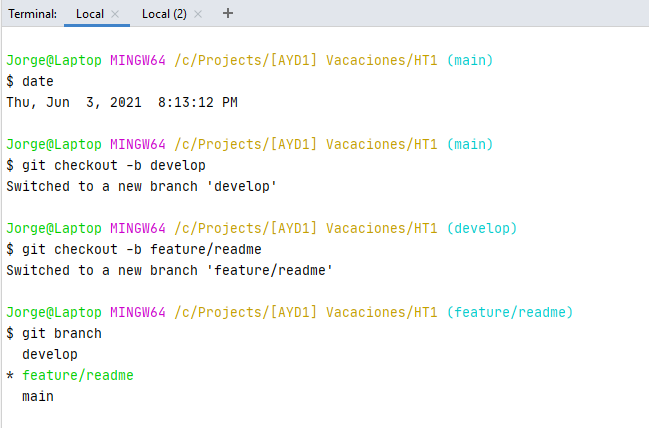
\includegraphics{1.PNG} \\\\
	\hrule
	\vspace{1cm}
	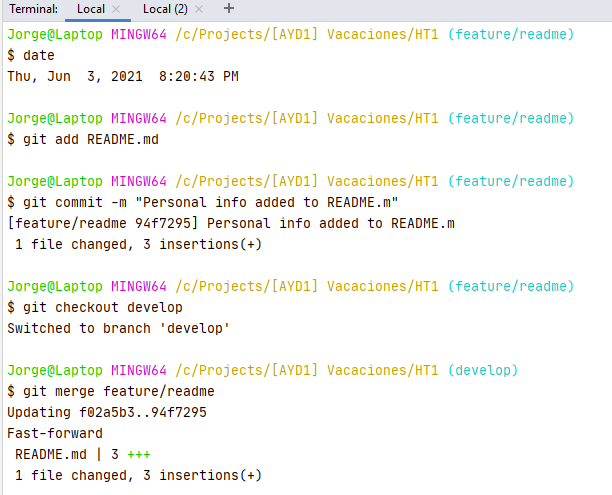
\includegraphics{2.PNG} \\\\
	\hrule
	\vspace{1cm}
	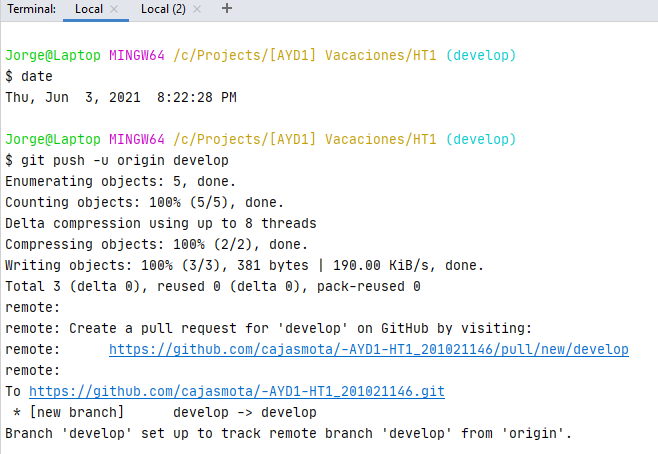
\includegraphics{3.PNG} \\\\
	\hrule
	\vspace{1cm}
	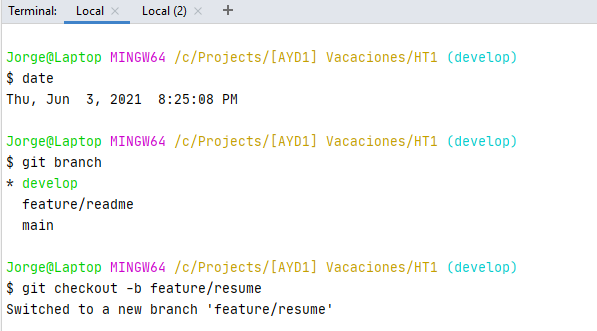
\includegraphics{4.PNG} \\\\
	\hrule
	\vspace{1cm}
	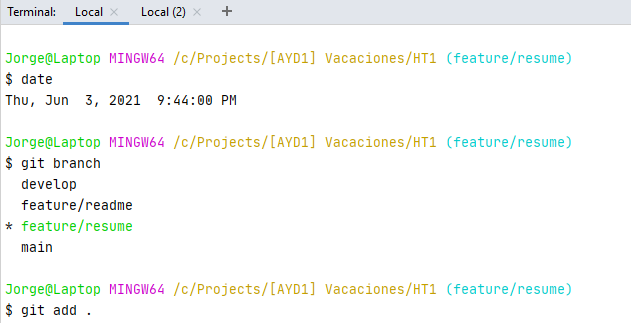
\includegraphics{5.PNG} \\\\
	\hrule 
	\vspace{1cm}
	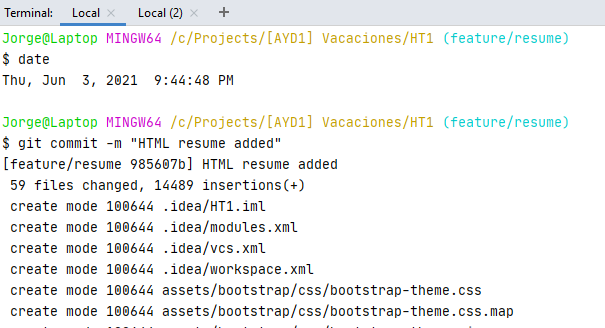
\includegraphics{6.PNG} \\\\
	\hrule 
	\vspace{1cm}
	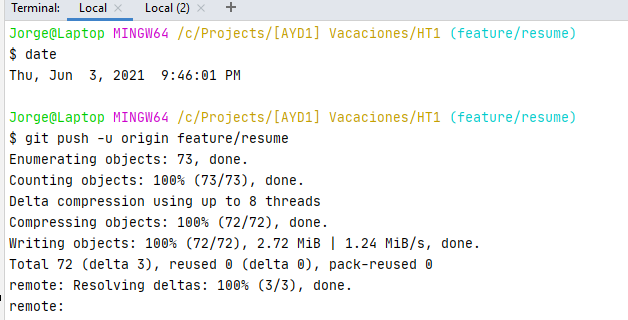
\includegraphics{7.PNG} \\\\
	\hrule 
	\vspace{1cm}
	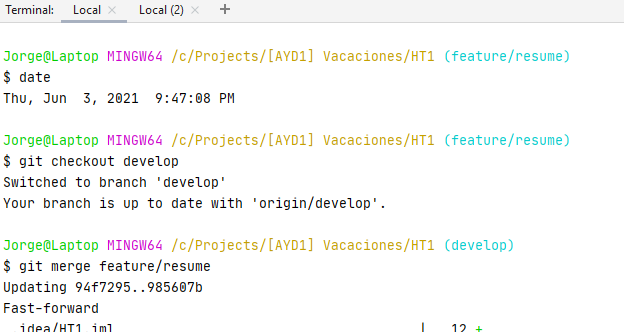
\includegraphics{8.PNG} \\\\
	\hrule 
	\vspace{1cm}
	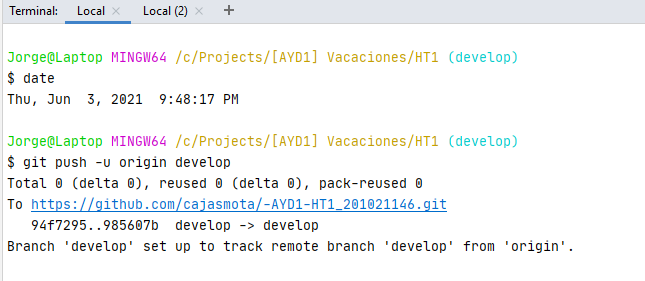
\includegraphics{9.PNG} \\\\
	\hrule 
	\vspace{1cm}
	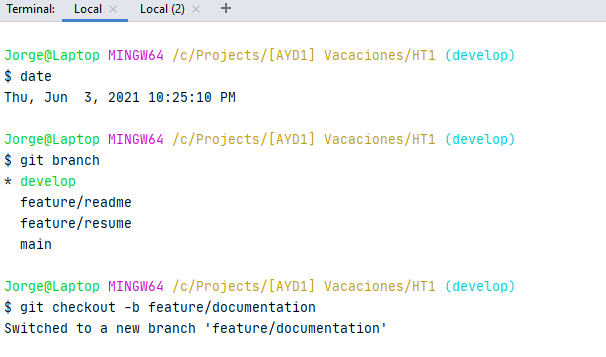
\includegraphics{10.PNG}
	\hrule 
	
	
\end{document}